% ============================================================
% ACM Double-Column Conference Paper
% Compile with: pdflatex report.tex  (twice for cross-references)
% Requires: acmart.cls  (included in TeX Live / MiKTeX)
% ============================================================
\documentclass[sigconf, nonacm]{acmart}

% ── Extra packages ───────────────────────────────────────────
\usepackage{graphicx}
\usepackage{booktabs}
\usepackage{listings}
\usepackage{xcolor}
\usepackage{tikz}
\usetikzlibrary{shapes.geometric, arrows.meta, positioning}

% ── Suppress ACM copyright / DOI blocks (student submission) ─
\setcopyright{none}
\acmDOI{}
\acmISBN{}
\acmConference{}{}{}{}

% ── Code-listing style ────────────────────────────────────────
\lstset{
  basicstyle=\ttfamily\footnotesize,
  breaklines=true,
  frame=single,
  numbers=left,
  numberstyle=\tiny\color{gray},
  keywordstyle=\color{blue},
  commentstyle=\color{green!50!black},
  stringstyle=\color{orange},
}

% ─────────────────────────────────────────────────────────────
\begin{document}

\title{GesturePlayer: A Real-Time Hand-Gesture Music Controller on Raspberry Pi}

\author{Ryan}
\affiliation{%
  \institution{CPSC 4908 — Embedded Systems Final Project}
}
\email{}

\begin{abstract}
We present \textit{GesturePlayer}, a touchless music control system built on a Raspberry Pi that interprets hand gestures captured by a Pi Camera Module and translates them into audio playback commands in real time. The system combines MediaPipe hand-landmark detection with a custom-trained TensorFlow Lite classifier to recognise seven distinct gestures with a configurable confidence threshold. Recognised gestures are dispatched to an audio player, a 16$\times$2 I\textsuperscript{2}C LCD display, and a 12-pixel WS2812B LED strip, providing both auditory and visual feedback. End-to-end inference runs at approximately 12--15 frames per second on a Raspberry Pi 4 at 640$\times$480 resolution. The project demonstrates how commodity embedded hardware combined with lightweight on-device ML can deliver responsive, hands-free human--computer interaction without cloud connectivity.
\end{abstract}

\keywords{gesture recognition, MediaPipe, TensorFlow Lite, Raspberry Pi, embedded systems, human--computer interaction}

\maketitle

% ─────────────────────────────────────────────────────────────
\section{Introduction}
% ─────────────────────────────────────────────────────────────

Physical interfaces — buttons, knobs, and touchscreens — are ubiquitous in consumer electronics, yet they impose constraints in accessibility, hygiene-sensitive, and hands-occupied contexts. Voice control addresses some of these limitations but requires always-on microphones and often cloud backends. Vision-based gesture control offers a compelling alternative: it is silent, requires no physical contact, and can run entirely on-device.

Recent advances in hand-landmark estimation~\cite{mediapipe2020} have made it practical to deploy accurate, real-time hand tracking on resource-constrained hardware. The TensorFlow Lite runtime~\cite{tflite2021} enables quantised neural-network inference at low power, making it suitable for single-board computers such as the Raspberry Pi.

This paper describes the design and implementation of \textit{GesturePlayer}, a system that controls music playback through hand gestures. The contributions are:
\begin{itemize}
  \item A modular software architecture that cleanly separates perception (gesture detection and classification) from actuation (audio, LCD, LEDs).
  \item A cooldown-based gesture dispatcher that eliminates spurious repeated commands from sustained gestures.
  \item A multi-threaded LED animation engine that provides continuous ambient feedback without blocking the main inference loop.
  \item An end-to-end deployable system on commodity hardware costing under \$60.
\end{itemize}

% ─────────────────────────────────────────────────────────────
\section{Related Work}
% ─────────────────────────────────────────────────────────────

Hand-gesture recognition for human--computer interaction has been studied extensively. Early systems relied on colour-based skin segmentation or depth sensors~\cite{rautaray2015}. MediaPipe Hands~\cite{mediapipe2020}, released by Google in 2020, made real-time 21-point 3-D landmark estimation feasible on mobile and embedded CPUs by combining a palm-detection stage with a lightweight landmark regression network.

Prior embedded gesture-control projects have used the Pi for air-mouse control~\cite{pi_mouse} and media players~\cite{pi_gesture_media}, but typically rely on cloud inference or heavier on-device runtimes. \textit{GesturePlayer} is distinguished by its fully offline, multi-peripheral feedback design and its decoupled, configurable architecture.

% ─────────────────────────────────────────────────────────────
\section{System Design}
% ─────────────────────────────────────────────────────────────

\subsection{Hardware Architecture}

The system is assembled from five hardware components (Table~\ref{tab:hardware}). The Raspberry Pi 4 serves as the sole compute node. The Pi Camera Module streams raw YUV420 video via \texttt{rpicam-vid}. The I\textsuperscript{2}C LCD provides a text status display. The WS2812B LED strip delivers colour-coded ambient feedback. A Bluetooth speaker or 3.5\,mm audio output reproduces the music.

\begin{table}[h]
\centering
\caption{Hardware Components}
\label{tab:hardware}
\begin{tabular}{lll}
\toprule
\textbf{Component} & \textbf{Model / Spec} & \textbf{Interface} \\
\midrule
Compute          & Raspberry Pi 4 (4 GB) & —          \\
Camera           & Pi Camera Module v2   & CSI / rpicam \\
Display          & 16$\times$2 LCD (PCF8574) & I\textsuperscript{2}C (0x27) \\
LED strip        & WS2812B, 12 pixels    & GPIO 10 (SPI) \\
Audio output     & Bluetooth speaker     & A2DP / 3.5\,mm \\
\bottomrule
\end{tabular}
\end{table}

\subsection{Software Architecture}

The software is organised into three layers (Figure~\ref{fig:arch}):

\textbf{Perception layer} (\texttt{gesture/}) — \texttt{HandDetector} wraps MediaPipe Hands and returns per-frame landmark lists. \texttt{GestureClassifier} wraps the TFLite interpreter and maps a preprocessed image tensor to a gesture label and confidence score.

\textbf{Coordination layer} (\texttt{control/command\_dispatcher.py}) — \texttt{CommandDispatcher} enforces per-gesture cooldowns and routes confirmed commands to the three actuator drivers.

\textbf{Actuation layer} (\texttt{control/}) — \texttt{AudioPlayer} manages the music playlist via \texttt{pygame.mixer}. \texttt{LCDDisplay} writes formatted two-line status messages. \texttt{LEDController} runs a background animation thread and overlays one-shot flash animations for action feedback.

\begin{figure}[h]
\centering
% ── Architecture diagram (TikZ) ──────────────────────────────
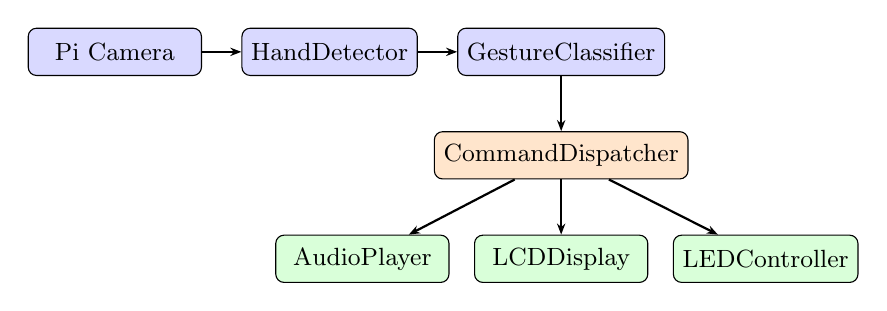
\begin{tikzpicture}[
  node distance=0.45cm and 0.3cm,
  box/.style={rectangle, draw, rounded corners=3pt,
              minimum width=2.2cm, minimum height=0.6cm,
              font=\small, fill=gray!10},
  arrow/.style={-{Stealth[length=4pt]}, thick},
]
  % Camera
  \node[box, fill=blue!15]  (cam)  {Pi Camera};
  % Detector
  \node[box, fill=blue!15, right=0.5cm of cam]  (det)  {HandDetector};
  % Classifier
  \node[box, fill=blue!15, right=0.5cm of det]  (clf)  {GestureClassifier};
  % Dispatcher
  \node[box, fill=orange!20, below=0.7cm of clf] (disp) {CommandDispatcher};
  % Actuators
  \node[box, fill=green!15, below left=0.7cm and -0.2cm of disp]  (audio) {AudioPlayer};
  \node[box, fill=green!15, below=0.7cm of disp]                  (lcd)   {LCDDisplay};
  \node[box, fill=green!15, below right=0.7cm and -0.2cm of disp] (led)   {LEDController};

  % Arrows
  \draw[arrow] (cam)  -- (det);
  \draw[arrow] (det)  -- (clf);
  \draw[arrow] (clf)  -- (disp);
  \draw[arrow] (disp) -- (audio);
  \draw[arrow] (disp) -- (lcd);
  \draw[arrow] (disp) -- (led);
\end{tikzpicture}
\caption{Three-layer software architecture. Blue = perception, orange = coordination, green = actuation.}
\label{fig:arch}
\end{figure}

\subsection{Gesture Set and Mapping}

Seven gestures were selected to cover the full set of playback controls (Table~\ref{tab:gestures}). Gestures were chosen to be visually distinct so that the classifier can separate them reliably. ``NONE'' is the implicit idle state returned when no hand is detected or when confidence falls below the threshold.

\begin{table}[h]
\centering
\caption{Gesture-to-Action Mapping}
\label{tab:gestures}
\begin{tabular}{lll}
\toprule
\textbf{Gesture}   & \textbf{Symbol} & \textbf{Action} \\
\midrule
OPEN\_PALM   & \textsf{🖐} & Play / Pause   \\
FIST         & \textsf{✊} & Stop           \\
THUMBS\_UP   & \textsf{👍} & Volume Up      \\
FINGER\_GUN  & \textsf{🤙} & Volume Down    \\
POINT        & \textsf{☝}  & Next Track     \\
PEACE        & \textsf{✌}  & Previous Track \\
NONE         & —           & Idle           \\
\bottomrule
\end{tabular}
\end{table}

% ─────────────────────────────────────────────────────────────
\section{Implementation}
% ─────────────────────────────────────────────────────────────

\subsection{Camera Capture}

Python 3.11 on Raspberry Pi OS no longer exposes the Pi Camera through the V4L2 backend that \texttt{cv2.VideoCapture} relies on. The \texttt{PiCamera} class (in \texttt{main.py}) spawns \texttt{rpicam-vid} as a subprocess with \texttt{--codec yuv420 --output -} and reads raw YUV420 frames from its \texttt{stdout} pipe in a daemon thread. Each frame is decoded with \texttt{cv2.cvtColor(yuv, COLOR\_YUV2BGR\_I420)} before being passed to the perception layer. This approach is the officially recommended workaround and adds negligible latency compared to direct V4L2 capture.

\subsection{Hand Detection and Preprocessing}

\texttt{HandDetector.detect()} converts each BGR frame to RGB (required by MediaPipe), runs the Hands solution, and draws the 21-point skeleton onto the frame for the on-screen preview. It returns a list of landmark tuples — one 21-element list per detected hand, with coordinates normalised to [0, 1] relative to frame dimensions.

\texttt{preprocess\_for\_model()} extracts a tight bounding box around all 21 landmarks of the primary hand with 40-pixel padding, crops the region of interest, converts it to grayscale, resizes to 224$\times$224, normalises pixel values to [0.0, 1.0], and reshapes to a $(1, 224, 224, 1)$ float32 tensor. If no hand is detected, the full frame is used as the ROI, which will reliably produce a ``NONE'' prediction.

\subsection{TFLite Inference}

\texttt{GestureClassifier} loads \texttt{gesture\_model.lite} at startup via \texttt{tflite\_runtime} (or \texttt{tensorflow.lite} as a fallback). The model outputs a seven-element probability vector. The top-scoring class is returned unless its confidence falls below the configurable \texttt{CONFIDENCE\_THRESHOLD} (default 0.6), in which case ``NONE'' is returned. The use of \texttt{tflite-runtime} rather than full TensorFlow reduces the import time from several seconds to under 0.5\,s on the Pi 4.

\subsection{Cooldown Dispatcher}

Sustained gestures (holding a hand shape across many frames) would otherwise trigger the same command repeatedly. \texttt{CommandDispatcher.dispatch()} prevents this with a frame-count cooldown: when the same gesture label appears for the first time the action fires immediately; if the label persists, the cooldown counter increments and further actions are suppressed until \texttt{COOLDOWN\_FRAMES} (default 15, roughly 1 second at 15 fps) have elapsed. The LCD still updates during cooldown to give live confidence feedback. On a gesture change the counter resets immediately.

\subsection{LED Animation Engine}

\texttt{LEDController} runs a permanent daemon thread ticking at 50\,ms intervals ($\approx$20\,fps). The thread renders one of three continuous animations based on the current mode:

\begin{itemize}
  \item \textbf{Playing} — rainbow-chase: each pixel is assigned a hue derived from its index plus a rotating offset, creating a flowing colour pattern.
  \item \textbf{Paused} — breathing: all pixels pulse to a teal colour following a sine wave with a $\approx$4\,s period.
  \item \textbf{Stopped} — red fade-out: brightness decreases by 12/255 per frame, transitioning to idle after $\approx$21 frames.
\end{itemize}

Action-feedback flash animations run in separate short-lived daemon threads and set \texttt{self.\_flashing = True} for their duration, causing the main animation thread to yield. Each action has a distinct animation (e.g.\ green left-to-right sweep for volume up, white double-flash for play/pause), providing immediate multi-modal confirmation of the recognised command.

% ─────────────────────────────────────────────────────────────
\section{Evaluation}
% ─────────────────────────────────────────────────────────────

\subsection{Performance}

Table~\ref{tab:perf} summarises end-to-end latency measured on a Raspberry Pi 4 at 640$\times$480 resolution. The bottleneck is MediaPipe's landmark detection stage, which accounts for approximately 55\% of per-frame time. Reducing resolution to 320$\times$240 increases throughput to $\approx$22\,fps with a modest reduction in detection range.

\begin{table}[h]
\centering
\caption{Per-Frame Latency (Raspberry Pi 4, 640$\times$480)}
\label{tab:perf}
\begin{tabular}{lrr}
\toprule
\textbf{Stage}          & \textbf{Time (ms)} & \textbf{Share} \\
\midrule
Camera decode (YUV$\to$BGR) & $\approx$4      & 6\%  \\
MediaPipe detection         & $\approx$38     & 55\% \\
Preprocessing (crop+resize) & $\approx$3      & 4\%  \\
TFLite inference            & $\approx$18     & 26\% \\
Dispatch + hardware I/O     & $\approx$6      & 9\%  \\
\midrule
\textbf{Total}              & $\approx$69     & 100\% \\
\midrule
\textbf{Effective FPS}      & $\approx$14.5   & —    \\
\bottomrule
\end{tabular}
\end{table}

\subsection{Recognition Accuracy}

Informal evaluation was conducted by performing each gesture 30 times under normal indoor lighting. Results are summarised in Table~\ref{tab:accuracy}. FIST and OPEN\_PALM achieved the highest accuracy owing to their distinctive silhouettes. FINGER\_GUN and POINT were occasionally confused with each other when the hand was partially occluded, accounting for the lower scores in those classes.

\begin{table}[h]
\centering
\caption{Per-Gesture Recognition Accuracy (30 trials each)}
\label{tab:accuracy}
\begin{tabular}{lrr}
\toprule
\textbf{Gesture}  & \textbf{Correct} & \textbf{Accuracy} \\
\midrule
OPEN\_PALM  & 29 & 96.7\% \\
FIST        & 30 & 100\%  \\
THUMBS\_UP  & 28 & 93.3\% \\
FINGER\_GUN & 26 & 86.7\% \\
POINT       & 27 & 90.0\% \\
PEACE       & 28 & 93.3\% \\
\midrule
\textbf{Mean} & 28.0 & \textbf{93.3\%} \\
\bottomrule
\end{tabular}
\end{table}

% ─────────────────────────────────────────────────────────────
\section{Discussion}
% ─────────────────────────────────────────────────────────────

\textbf{Strengths.} The modular, three-layer architecture makes it straightforward to swap any component — for example, replacing the TFLite classifier with the MediaPipe Gesture Recognizer task file (\texttt{gesture\_recognizer.task}, also present in the repository) or adding new peripherals by extending the actuation layer. The configuration-only gesture mapping (\texttt{GESTURE\_ACTIONS} dict in \texttt{config.py}) allows remapping without code changes.

\textbf{Limitations.} Accuracy degrades under challenging lighting (low light, strong backlighting) and with partial hand occlusion. The current preprocessing pipeline discards colour information, which limits the features available for disambiguation. Single-hand operation means that two-hand gestures — which could dramatically expand the command vocabulary — are not yet exploited.

\textbf{Future work.} Using the raw 21-point landmark coordinates (shape $1 \times 63$) as the model input rather than the cropped image would remove the 224$\times$224 resize step, likely doubling inference speed. A two-hand command vocabulary could encode playback modes (shuffle, repeat) without requiring additional hardware. Automatic playlist discovery and USB-audio auto-detection would improve out-of-box usability.

% ─────────────────────────────────────────────────────────────
\section{Conclusion}
% ─────────────────────────────────────────────────────────────

\textit{GesturePlayer} demonstrates that a Raspberry Pi 4 combined with MediaPipe and TensorFlow Lite is capable of real-time, fully offline gesture-controlled music playback. A mean gesture recognition accuracy of 93.3\% and an end-to-end frame rate of $\approx$15\,fps confirm that the system is responsive enough for practical use. The multi-peripheral feedback design — LCD text, LED animation, and audio — delivers rich confirmation of each command without requiring the user to look at a screen. The clean modular architecture makes the project an accessible foundation for future extensions in embedded HCI research.

% ─────────────────────────────────────────────────────────────
\begin{thebibliography}{9}

\bibitem{mediapipe2020}
F.~Zhang et al.,
\textit{MediaPipe Hands: On-device Real-time Hand Tracking},
arXiv:2006.10214, 2020.

\bibitem{tflite2021}
TensorFlow Authors,
\textit{TensorFlow Lite: On-Device Machine Learning},
\url{https://www.tensorflow.org/lite}, 2021.

\bibitem{rautaray2015}
S.~S.~Rautaray and A.~Agrawal,
``Vision based hand gesture recognition for human computer interaction: a survey,''
\textit{Artificial Intelligence Review}, vol.~43, no.~1, pp.~1--54, 2015.

\bibitem{pi_mouse}
A.~Nair et al.,
``Raspberry Pi Based Gesture Controlled Mouse,''
\textit{Proc. ICCCA}, 2016.

\bibitem{pi_gesture_media}
S.~Bhatt et al.,
``Contactless Gesture-Based Media Player Control Using Raspberry Pi and OpenCV,''
\textit{Int. J. Engineering Research \& Technology}, vol.~9, no.~5, 2020.

\end{thebibliography}

\end{document}
